\documentclass[conference]{IEEEtran}
\IEEEoverridecommandlockouts

\usepackage{cite}
\usepackage{amsmath,amssymb,amsfonts}
\usepackage{graphicx}
\graphicspath{{../figures/}{figures/}}
\usepackage{textcomp}
\usepackage{booktabs}
\usepackage{url}
\usepackage{xcolor}
\def\BibTeX{{\rm B\kern-.05em{\sc i\kern-.025em b}\kern-.08em
    T\kern-.1667em\lower.7ex\hbox{E}\kern-.125emX}}

\raggedbottom

\begin{document}

\title{Empirical Audit of a Preprocessing Strategy for\\
Food Price Spike Prediction in Nigerian States}

\author{\IEEEauthorblockN{Nimat Ohunene Sadiq}
\IEEEauthorblockA{\textit{Carnegie Mellon University Africa} \\
Kigali, Rwanda \\
nsadiq@andrew.cmu.edu}}

\maketitle

\begin{abstract}
This report audits a preprocessing and feature engineering strategy against its
implementation. The system predicts, one month ahead, whether the price of a
staple food in a Nigerian state will exceed its trailing three-month mean by
more than 15\%. Execution produced six documented deviations from the planned
design, each driven by a measured property of the data rather than by
convenience. Little's test rejected the MCAR hypothesis
($\chi^2 = 6894.23$, $df = 365$, $p < 0.001$), confirming that gaps in market
reporting carry signal and must be encoded rather than imputed away. Price
levels exhibited extreme right skew (skewness $= 23.47$, kurtosis $= 855.83$),
yet values flagged by a Tukey fence preceded a spike in 21.4\% of cases against
a 16.3\% base rate, so winsorization was rejected as signal destruction. A
pairwise correlation screen flagged one feature pair at
$\rho = 0.876$, while variance inflation independently flagged a feature the
pairwise screen missed (VIF $= 10.52$); removing it reduced maximum VIF to
6.72. All fitted transformations are encapsulated in \texttt{Pipeline} and
\texttt{ColumnTransformer} objects and fitted on the training partition alone;
an injected future feature raised test ROC-AUC to 1.000 against 0.738 for the
production pipeline, verifying that the harness detects leakage. The final
design matrix retains 16 features from 32 panel columns with no information
loss.
\end{abstract}

\begin{IEEEkeywords}
preprocessing, data leakage, class imbalance, MNAR missingness, time series
classification, food security
\end{IEEEkeywords}

\section{Introduction}

Nigerian state governments and relief agencies learn that staple food prices
have risen only after the rise has occurred, because every published price
series is retrospective. Support therefore reaches households after they have
reduced consumption or sold assets, and public procurement happens at peak
prices. The system described here predicts a sharp price increase one month
ahead, producing a ranked monthly warning list.

The prediction target is binary: for each (state, commodity, month) triple,
$y = 1$ when the price in month $t+1$ exceeds its trailing three-month mean by
more than 15\%. The data source is the World Food Programme price database for
Nigeria, distributed through the Humanitarian Data Exchange, retrieved 3
October 2026.

This report is an audit rather than a description. Section~\ref{sec:dims}
verifies the matrix dimensions through each transformation stage.
Sections~\ref{sec:missing} through~\ref{sec:dim} present the statistical
evidence behind each preprocessing decision, cross-referencing the diagnostic
figures. Section~\ref{sec:leak} documents the leakage architecture and its
verification. Section~\ref{sec:log} summarises the planned strategy against
what execution required.

\section{Pipeline Output Verification}
\label{sec:dims}

The distributed file is not the matrix a model trains on, and conflating the
two misstates every missingness and imbalance figure. Table~\ref{tab:dims}
tracks dimensions through each stage.

\begin{table}[htbp]
\caption{Matrix dimensions through the pipeline}
\begin{center}
\begin{tabular}{@{}lrr@{}}
\toprule
\textbf{Stage} & \textbf{Rows ($N$)} & \textbf{Cols ($P$)} \\
\midrule
Raw file, long format & 88{,}545 & 16 \\
Panel (state $\times$ commodity $\times$ month) & 9{,}000 & 32 \\
Labelled rows & 6{,}940 & 32 \\
\midrule
Training partition & 4{,}956 & 32 \\
Validation partition & 1{,}075 & 32 \\
Test partition & 909 & 32 \\
\midrule
Design matrix, linear model & 4{,}956 & \textbf{16} \\
Design matrix, tree model & 4{,}956 & \textbf{17} \\
\bottomrule
\end{tabular}
\label{tab:dims}
\end{center}
\end{table}

The reduction from 32 panel columns to 16 model features involves no
information loss. The 16 removed columns comprise identifiers
(\texttt{state}, \texttt{commodity}, \texttt{month}), intermediate quantities
consumed by downstream features (\texttt{price\_lag1}, \texttt{roll\_mean\_6},
\texttt{trail\_mean}), label construction columns that must never reach the
model (\texttt{price\_next}), two features found to be structurally constant
(Section~\ref{sec:missing}), and one removed by variance inflation
(Section~\ref{sec:collin}). The tree model retains 17 features because
collinearity reduction is applied only to the linear model.

The row reduction from 9{,}000 to 6{,}940 is also structural: the label
requires three prior months to form a trailing mean, so the first observations
of each of the 107 series cannot be labelled.

\section{Missingness Mechanism}
\label{sec:missing}

\subsection{The raw file contains no missing values}

A naive audit reports zero null cells across all 88{,}545 rows and 16 columns.
This is a reporting artefact rather than an absence of missingness: the
provider publishes only observed records, so a market that fails to report
produces no row at all. Missingness exists as absent \emph{rows} and becomes
visible only after reindexing each series onto a continuous monthly grid, at
which point 1{,}132 of 9{,}000 cells (12.58\%) are gaps. The gap rate differs
sharply by state: 26.27\% in Adamawa, 11.11\% in Borno, 7.88\% in Yobe.

Treating the zero-null finding as "no imputation required" would be a
substantive error, and it is the first finding the diagnostic pipeline is
designed to prevent.

\subsection{MCAR is rejected}

Little's test was applied to the 14 continuous training features across 35
distinct missingness patterns. The statistic was
$\chi^2 = 6894.23$ on $df = 365$, $p < 0.001$, rejecting the hypothesis that
data are missing completely at random.

Rejecting MCAR does not by itself distinguish MAR from MNAR, so association
tests were used to characterise the structure. Cram\'{e}r's $V$ was computed
between the gap indicator and each categorical variable
(Table~\ref{tab:cramers}). Effect sizes are reported alongside $\chi^2$ because
significance is inflated at this sample size.

\begin{table}[htbp]
\caption{Association between gap pattern and categorical variables}
\begin{center}
\begin{tabular}{@{}lrrl@{}}
\toprule
\textbf{Variable} & \textbf{Cram\'{e}r's $V$} & \textbf{$\chi^2$} & \textbf{$p$} \\
\midrule
State & 0.1986 & 356.77 & $3.4\times10^{-78}$ \\
Commodity & 0.1131 & 150.01 & $3.4\times10^{-16}$ \\
Calendar month & 0.1127 & 125.21 & $1.6\times10^{-21}$ \\
Food type & 0.0039 & 1.13 & $0.287$ \\
\bottomrule
\end{tabular}
\label{tab:cramers}
\end{center}
\end{table}

State shows the strongest association, which matches the generating mechanism:
markets suspend reporting during insecurity, and insecurity is
geographically concentrated. Food type shows no association ($p = 0.287$),
confirming that gaps are not a property of what is being sold. Because markets
stop reporting under the same conditions that drive prices upward, missingness
depends on the unobserved value itself, which is the MNAR case.

\subsection{Consequences for imputation}

Figure 1.1 (missingness heatmap) shows gaps clustered in time and by series
rather than scattered. Three rules follow.

First, gaps are encoded rather than erased: a binary indicator and a six-month
gap count enter the feature set. Second, interpolation is restricted to
single-month gaps, of which 356 were filled and flagged; bridging a longer
silence would fabricate a smooth price path through precisely the period most
likely to contain a spike. Third, where a central value is required when
collapsing markets within a state, the \emph{median} is used, because
market-level prices are right-skewed and a single besieged market can print
several times the state norm.

\textbf{Deviation 1.} The planned design specified four missingness
indicators. Two, \texttt{is\_gap} and \texttt{months\_since\_obs}, proved
structurally constant within the modelling set: a gap month has no price,
therefore no trailing mean, therefore no label, and is never a modelled row.
Both were removed. The MNAR signal survives through \texttt{gaps\_last\_6m}
and \texttt{price\_was\_interpolated}, which describe gaps in a row's recent
history rather than in the row itself. The mechanism diagnosis was correct; the
assumption that a correct diagnosis yields usable features was not.

\section{Outlier Treatment}
\label{sec:outlier}

\subsection{Distribution shape dictates the rule}

Training price levels are extremely right-skewed: skewness $= 23.47$, kurtosis
$= 855.83$, with mean 588.16 NGN against median 400.00 NGN. The $Z$-score rule
assumes approximate normality and a stable mean, neither of which holds, so the
Tukey IQR fence was used, computed on the training partition only.

For price levels: $Q_1 = 198.0$, $Q_3 = 839.0$, $IQR = 641.0$, giving an upper
fence of 1800.5 NGN and flagging 140 values (2.82\% of training rows).

\subsection{Capping is rejected, with evidence}

The conventional treatment is winsorization at the fence. That would be
destructive here, and the measurement shows why.

Of the 140 flagged price values, 30 precede a spike. That is a 21.4\% spike
rate among flagged values against a 16.3\% training base rate. Extreme values
are therefore \emph{more} likely than ordinary values to precede the event
being predicted. Since the label is derived from the price series, capping
prices would flatten the largest movements and delete positive cases from the
training data, training the model to predict a phenomenon partly removed from
its view.

The IQR screen is consequently used diagnostically rather than correctively.
Flagged values are triaged: physically implausible readings are corrected or
treated as gaps, while extreme but plausible values are retained unchanged.

\begin{figure}[htbp]
\centerline{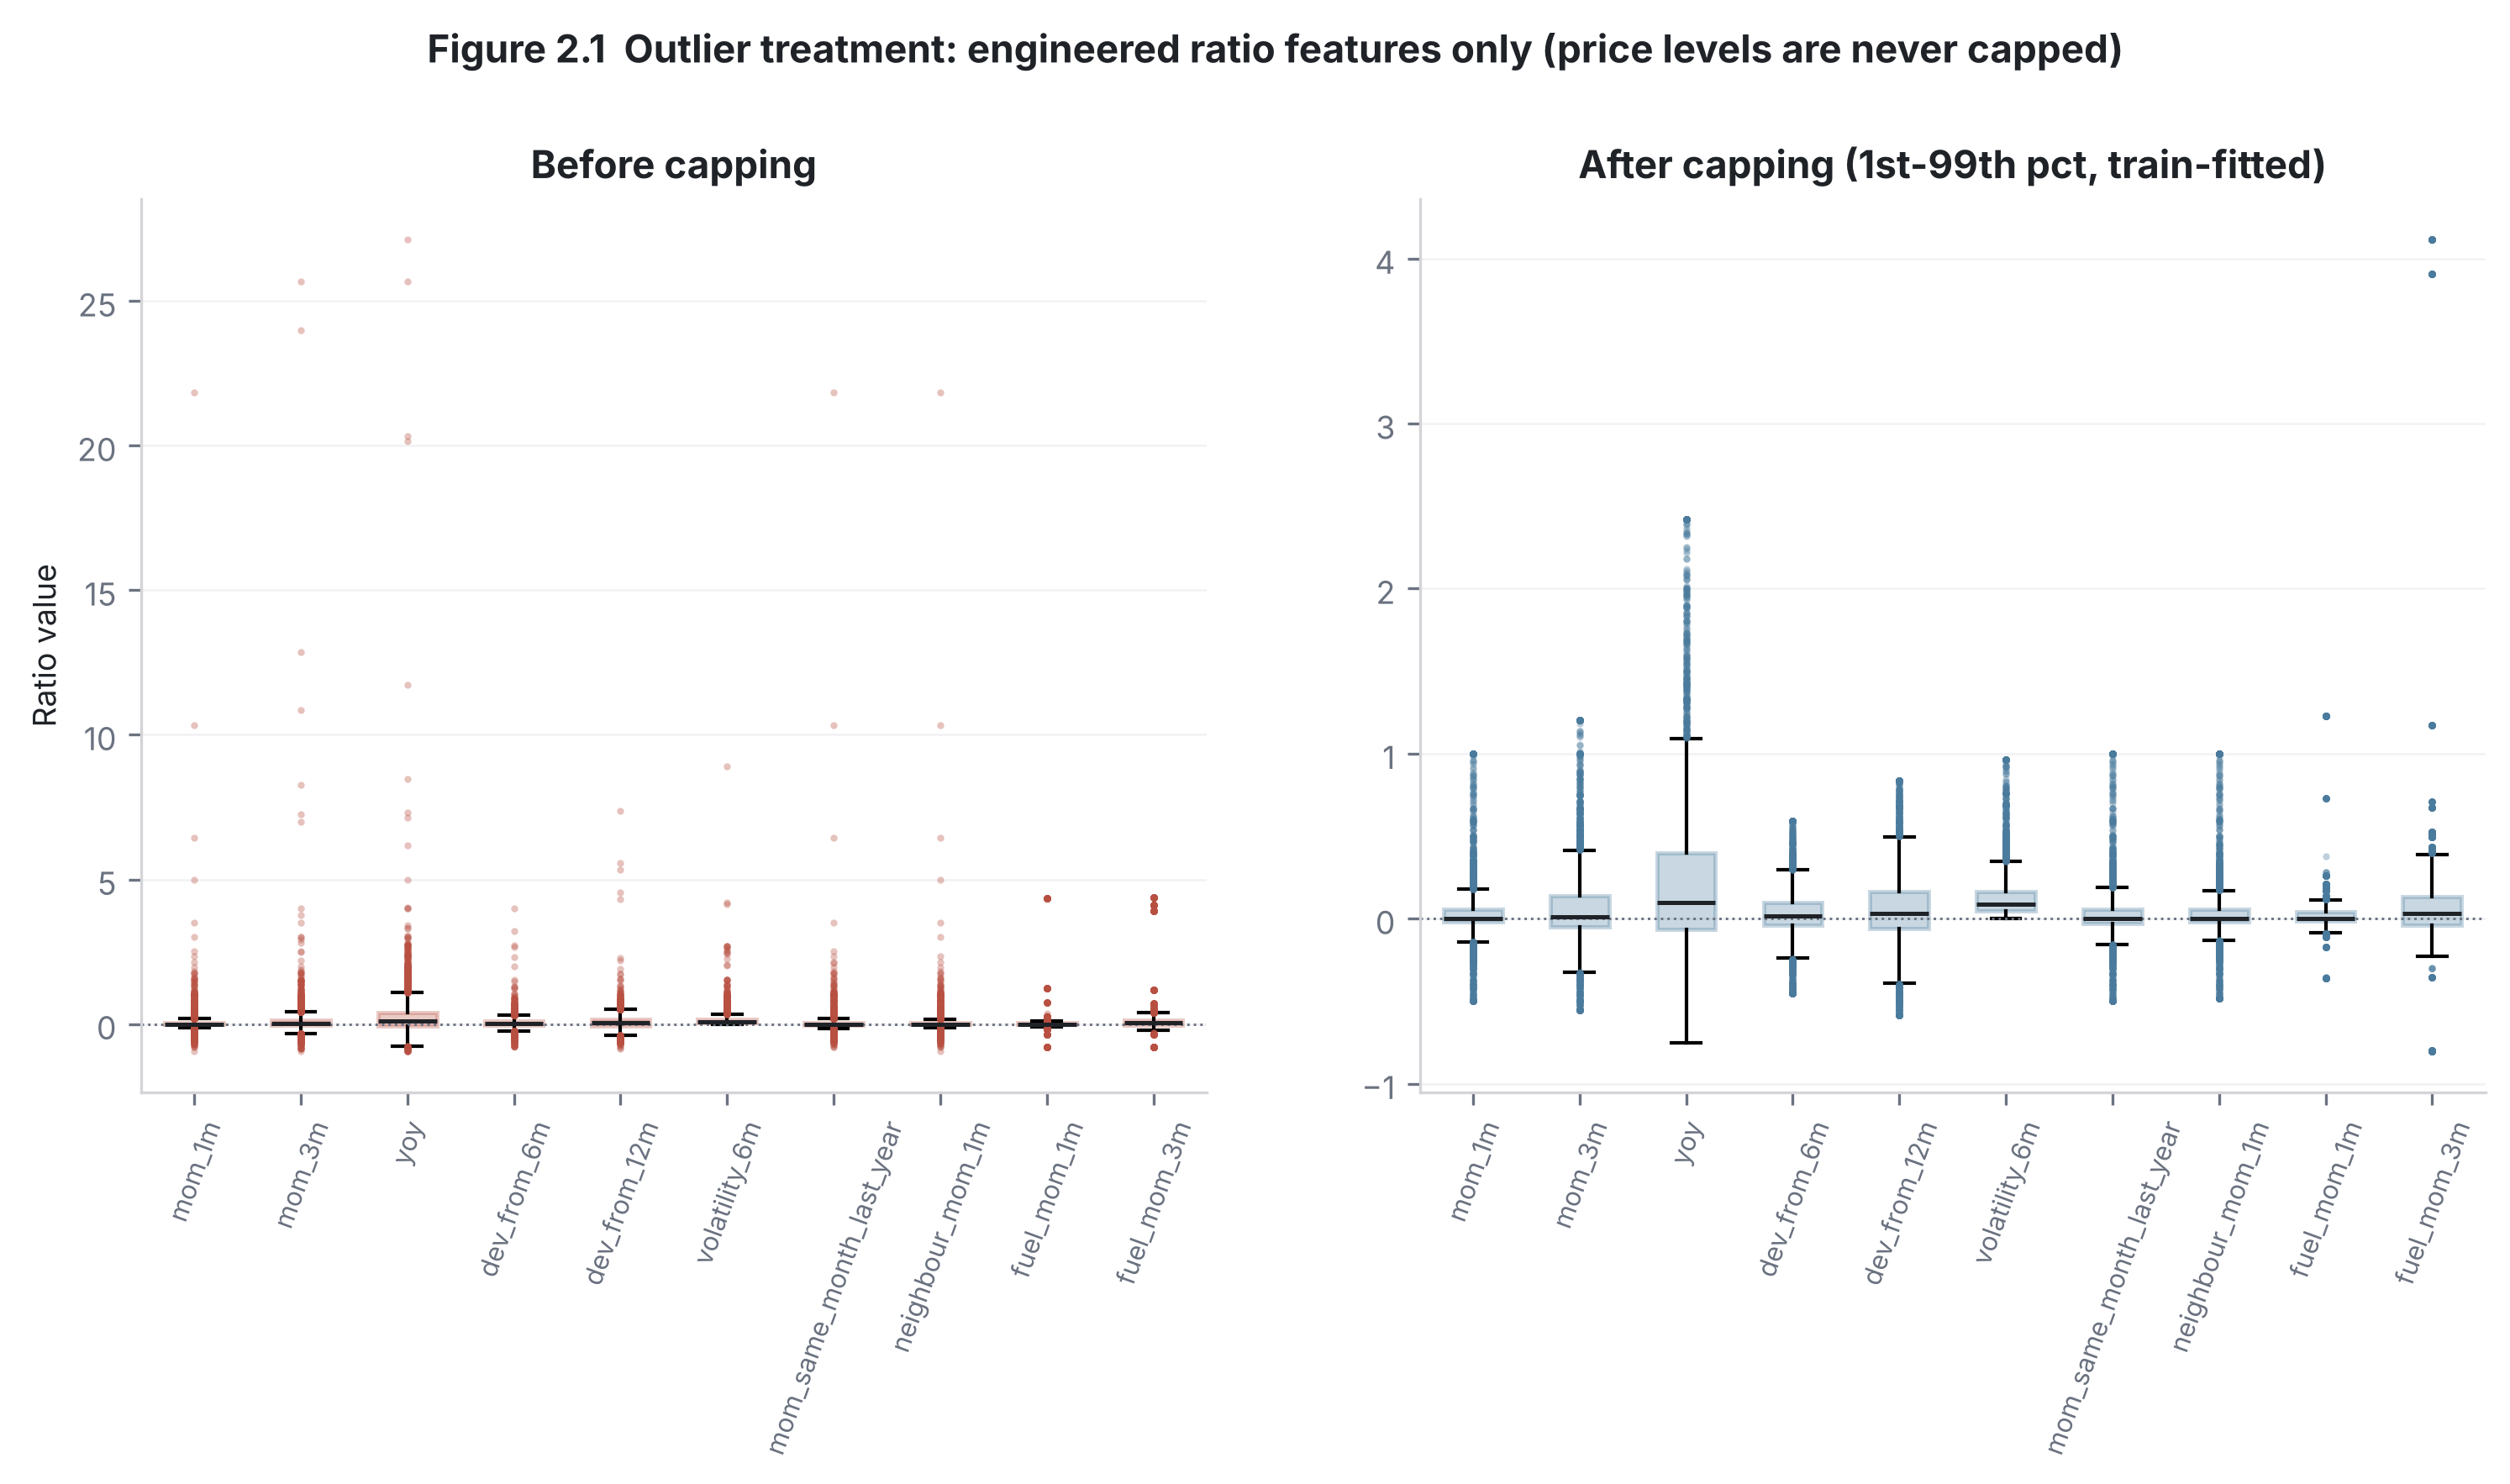
\includegraphics[width=\columnwidth]{fig2_1_outlier_boxplots.png}}
\caption{Ratio features before and after percentile capping. Price levels are
deliberately absent: capping them would delete positive cases, as the flagged
spike rate in Section~\ref{sec:outlier} shows.}
\label{fig:outlier}
\end{figure}

\subsection{Where capping does apply}

Engineered ratio features are a different case. A month-on-month ratio computed
across a long gap can produce an arbitrary multiple, which is an artefact of
construction rather than observed behaviour. These are capped at the 1st and
99th training percentiles. Table~\ref{tab:ratio} gives the shape statistics
justifying this, and Figure 2.1 shows the distributions before and after.

\begin{table}[htbp]
\caption{Ratio feature shape and fence bounds (training)}
\begin{center}
\begin{tabular}{@{}lrrr@{}}
\toprule
\textbf{Feature} & \textbf{Skew} & \textbf{Kurtosis} & \textbf{Flagged} \\
\midrule
\texttt{mom\_1m} & 32.72 & 1548.34 & 16.12\% \\
\texttt{dev\_from\_6m} & 4.33 & 65.39 & 9.67\% \\
\texttt{volatility\_6m} & 13.22 & 347.84 & 9.08\% \\
\bottomrule
\end{tabular}
\label{tab:ratio}
\end{center}
\end{table}

Figure 2.1 deliberately shows ratio features rather than price levels. A
reader expecting a raw-versus-capped price comparison should read this section
as the explanation for its absence.

\section{Transformation and Scaling}
\label{sec:transform}

Figure 4.1 tracks the price feature through the transformation chain. Applying
$\log(1+x)$ reduced skewness from $23.47$ to $-0.214$ and kurtosis from
$855.83$ to $-0.349$, producing a near-symmetric distribution. The IQR screen
in Section~\ref{sec:outlier} is applied on the log scale for the same reason.

Most engineered features are already ratios or proportional changes and are
approximately stationary, requiring no further transformation. This is
deliberate: modelling relative movement rather than absolute naira prices
allows a single pooled model to span commodities with different units and
price levels, and blunts the currency-driven level shifts of 2023 and 2024.

Scaling is matched to the estimator rather than applied uniformly.
\texttt{StandardScaler} is applied for logistic regression, because $L_2$
penalties shrink coefficients in proportion to feature magnitude and unscaled
inputs would be penalised differently purely because of units. No scaling is
applied for gradient boosted trees, which split on rank order and are invariant
to monotonic rescaling; adding a scaler would introduce a fitted step with no
benefit and one further opportunity for leakage.

\texttt{MinMaxScaler} was rejected. It is bounded by the training range and
acutely sensitive to outliers, which are deliberately retained here
(Section~\ref{sec:outlier}). The series is also non-stationary: 2026 prices
exceed anything in the 2016 training range, so test values would fall outside
$[0,1]$ regardless.

\section{Multicollinearity Screening}
\label{sec:collin}

\textbf{Deviation 2.} The planned design anticipated severe collinearity "by
construction", on the reasoning that momentum over one and three months share a
term. The pairwise screen did not support this. At $|\rho| \geq 0.85$
(Spearman, chosen over Pearson because of the skew documented in
Section~\ref{sec:outlier}), exactly one pair flagged across 14 features:
\texttt{mom\_3m} with \texttt{dev\_from\_6m} at $\rho = 0.876$
(Figure 3.1, Figure 3.2). Lagged \emph{ratios} at different horizons prove
less redundant than overlapping level windows would be.

Variance inflation then identified a feature the pairwise screen had missed.
\texttt{dev\_from\_12m} returned VIF $= 10.52$, exceeding the threshold,
despite no single pairwise correlation reaching $0.85$
(Table~\ref{tab:vif}). This is the case the two-stage protocol exists to
catch: a feature can be jointly predictable from several others without being
strongly correlated with any one of them.

\begin{table}[htbp]
\caption{Variance inflation factors (training)}
\begin{center}
\begin{tabular}{@{}lr@{}}
\toprule
\textbf{Feature} & \textbf{VIF} \\
\midrule
\texttt{dev\_from\_12m} & \textbf{10.52} \\
\texttt{dev\_from\_6m} & 8.33 \\
\texttt{mom\_3m} & 6.72 \\
\texttt{yoy} & 3.70 \\
\texttt{mom\_1m} & 3.58 \\
\texttt{volatility\_6m} & 2.59 \\
\bottomrule
\end{tabular}
\label{tab:vif}
\end{center}
\end{table}

The resolution rule compares mutual information against the target
(Figure 3.3): \texttt{dev\_from\_6m} scores $0.0636$ against
\texttt{dev\_from\_12m} at $0.0353$, so the latter was dropped. Maximum VIF
fell from $10.52$ to $6.72$, below threshold.

\begin{figure}[htbp]
\centerline{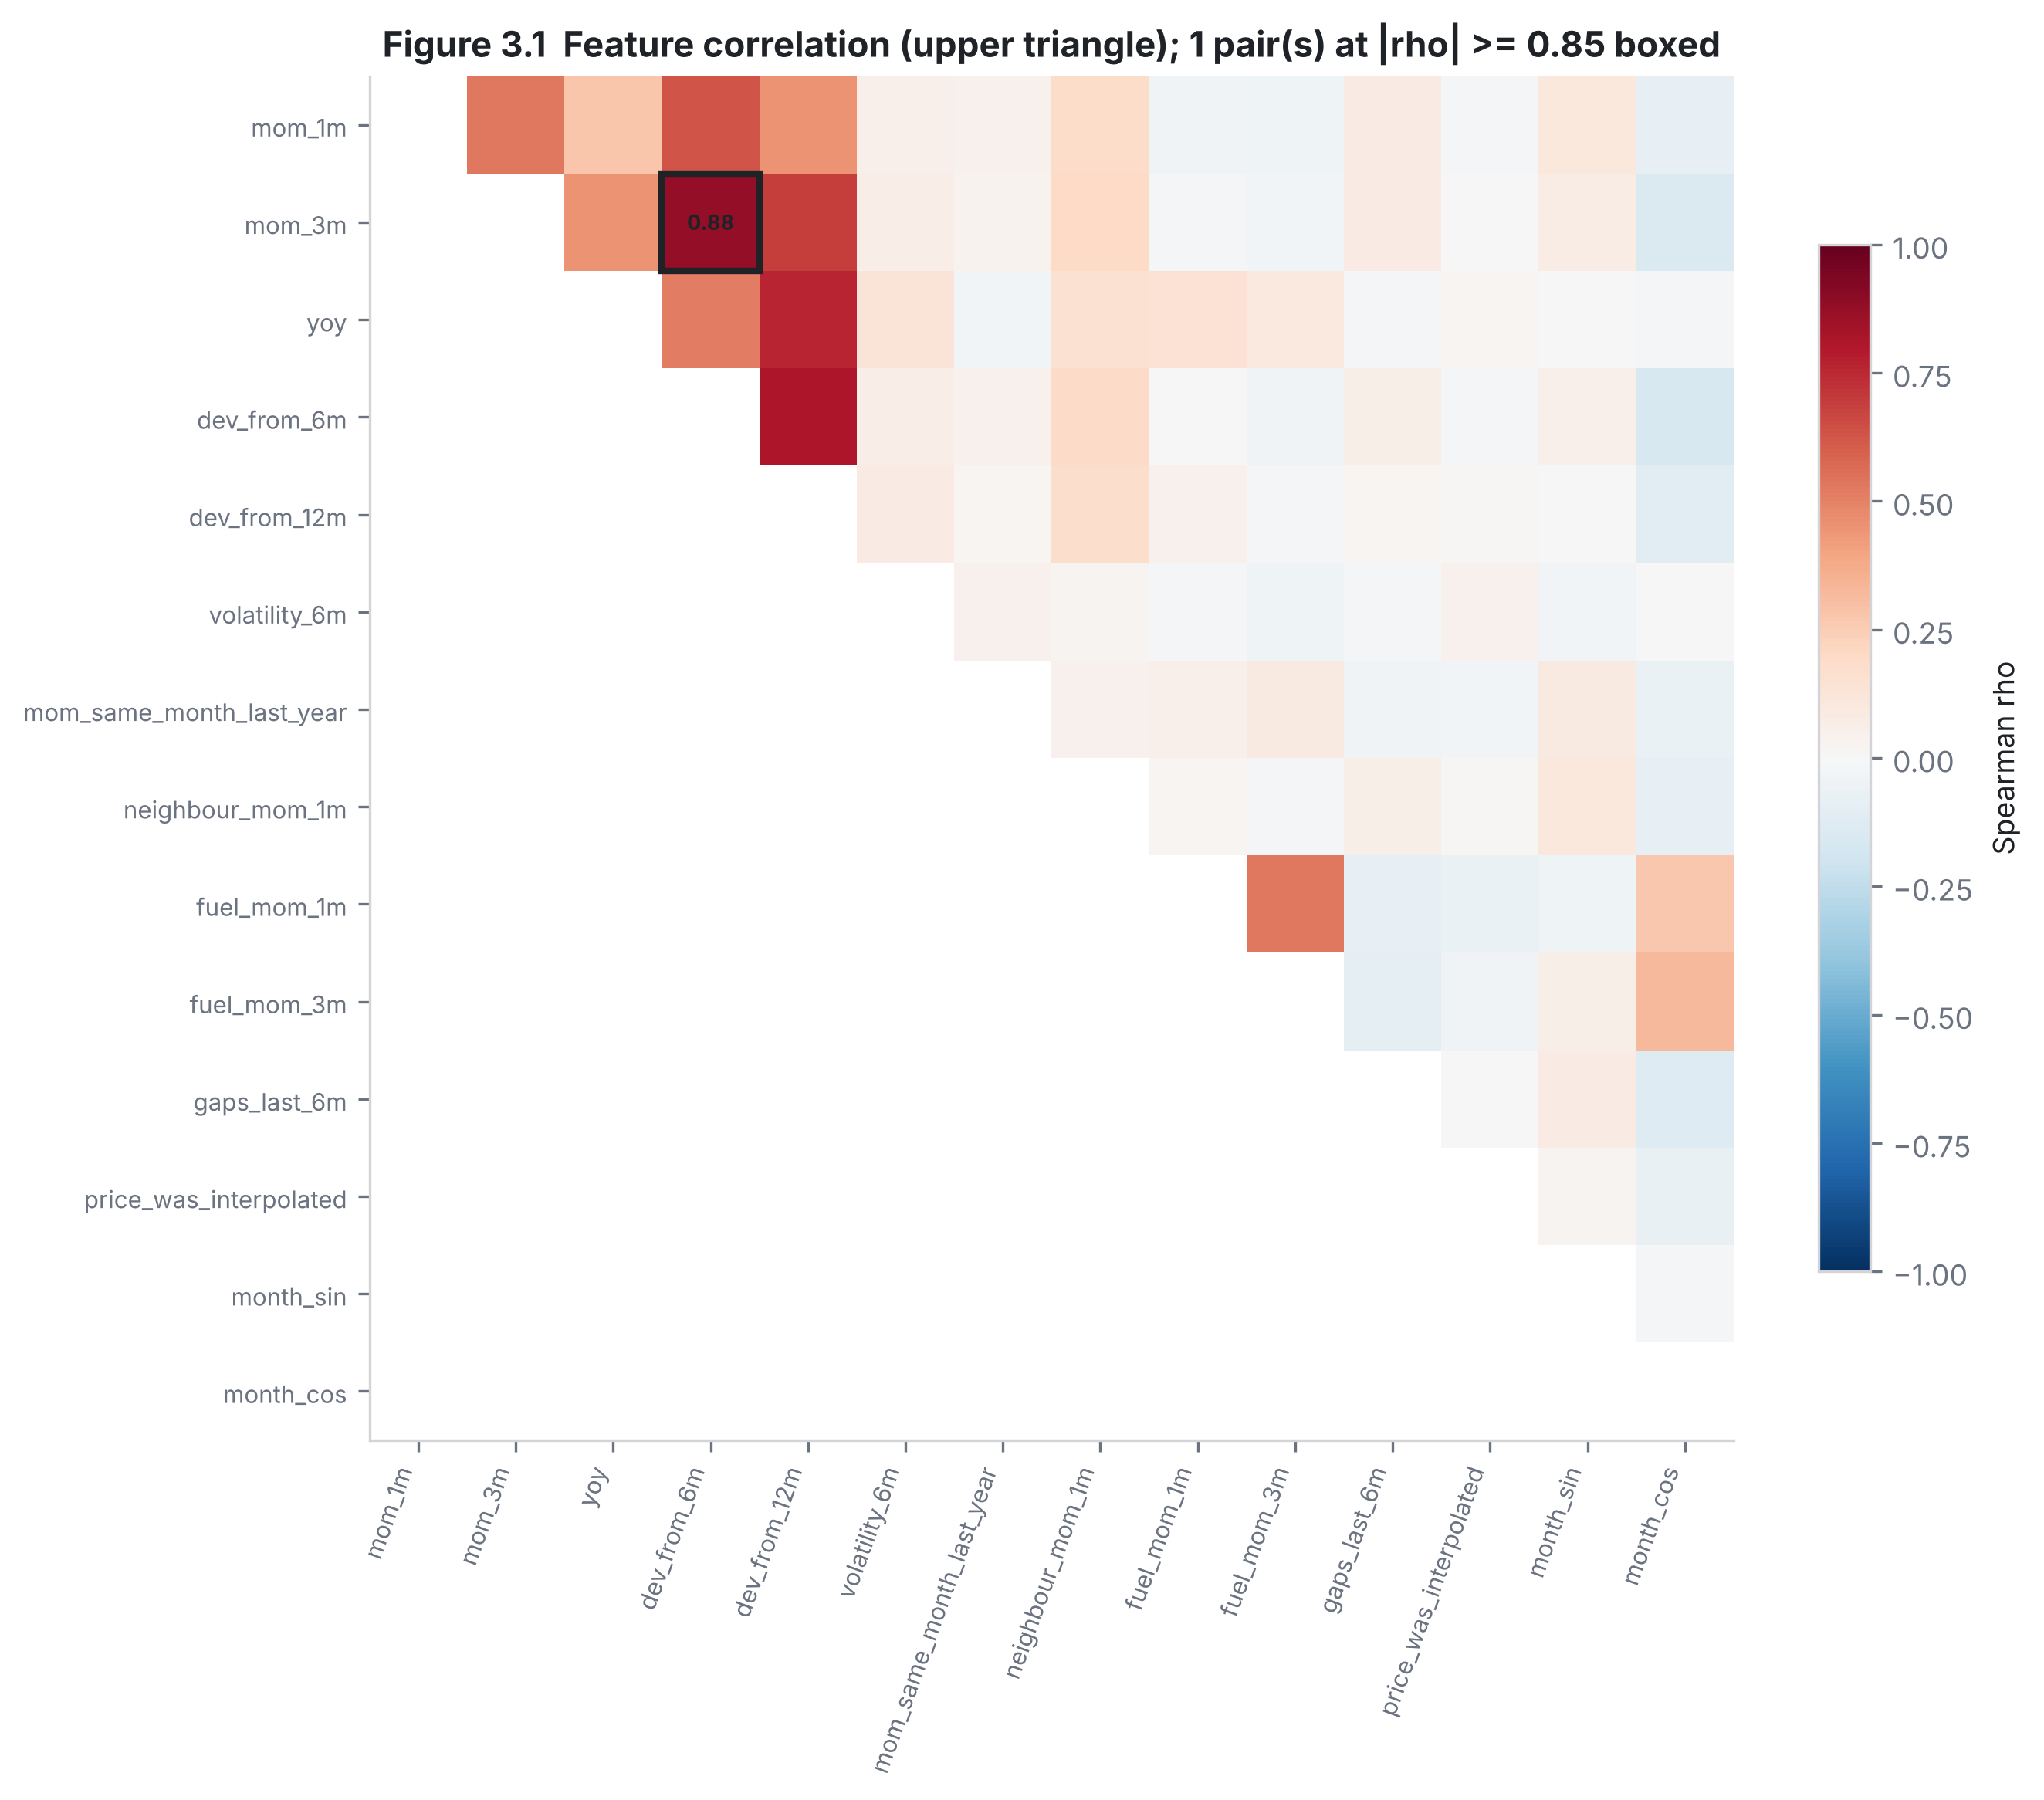
\includegraphics[width=\columnwidth]{fig3_1_correlation_matrix.png}}
\caption{Upper-triangle Spearman correlation on the training partition. One
pair exceeds the $0.85$ threshold. The feature removed from the linear model
was identified by variance inflation, not by this screen.}
\label{fig:corr}
\end{figure}

The reduced set is applied to logistic regression only. Collinearity
destabilises linear coefficients and makes them uninterpretable, which matters
because the linear model exists to be interpreted. Tree ensembles are not
destabilised by correlated inputs, so applying one rule to both estimators
would discard usable signal from the model able to exploit it. This accounts
for the 16-versus-17 feature difference in Table~\ref{tab:dims}.

\section{Dimensionality}
\label{sec:dim}

Principal component analysis was conducted on the 14-feature standardised
training matrix for diagnostic purposes (Figure 5.1). The first component
explains 29.63\% of variance (eigenvalue $4.149$); ten components are required
to reach 90\% of cumulative variance and eleven to reach 95\%.

\textbf{Deviation 3.} This result contradicts the planned expectation. The
original strategy predicted that PCA would be dominated by collinear lag
features and that the first component would absorb most of the variance. At
29.63\% it does not, and requiring ten of fourteen components for 90\% variance
indicates the feature set is close to full rank. This is consistent with
Section~\ref{sec:collin}: the features are less redundant than assumed.

PCA was accordingly not adopted as a transformation. It offers little
compression here, and components would destroy the coefficient
interpretability that justifies retaining a linear model at all.

\section{Leakage Prevention and Verification}
\label{sec:leak}

\subsection{Architecture}

Every fitted transformation is encapsulated within a \texttt{Pipeline} inside a
\texttt{ColumnTransformer}, so that \texttt{fit} is structurally unable to
touch held-out data. Imputation values, IQR capping bounds, scaler statistics
and the probability calibration mapping are all learned on the training
partition and applied unchanged to validation and test.

Partitioning is forward chronological: training 2016-03 to 2023-06, validation
2023-07 to 2024-12, test 2025-01 to 2026-06. Random splitting is inadmissible
because the dataset contains repeated observations of shared entities: each
(state, commodity) pair is one series observed monthly for up to 127 months,
and price series are autocorrelated, so a randomly held-out month sits between
two training months that nearly determine it.

A chronological boundary is simultaneously group-respecting, because no series
can appear on both sides of a date cut; \texttt{GroupKFold} is subsumed rather
than omitted. Within the training period, validation uses
\texttt{TimeSeriesSplit} with an expanding window.

Stratification is deliberately not applied. It requires reshuffling, which
would destroy the temporal ordering the design exists to respect. Class balance
per partition is reported instead (Section~\ref{sec:results}).

Publication lag is respected: official prices for a month are released around
the middle of the following month, so features are restricted to data that
would have been published by the prediction date.

\subsection{Verification by negative control}

A feature constructed from month $t+1$ was deliberately injected into the
feature set and the pipeline refitted. Test ROC-AUC rose to $1.000$ against
$0.738$ for the production pipeline. A harness unable to detect injected
leakage cannot be trusted to rule it out, so this control is reported rather
than assumed. The control feature was subsequently removed.

\textbf{Deviation 4.} The planned design committed to rebuilding lag features
inside every cross-validation fold, describing this as the subtlest available
leak. Implementation showed the reasoning to be over-cautious for this
construction. Every window looks strictly backwards from month $t$ and the
label is built from month $t+1$, so a training row at time $t$ touches only
months at or before $t$, all of which precede the split boundary. The
requirement binds for anything that \emph{learns a parameter}, and those steps
are inside the \texttt{Pipeline}; it does not bind for deterministic
backward-only windows under a chronological split. Conflating the two cases
produces either leakage or unnecessary complexity.

\section{Class Imbalance and Calibration}
\label{sec:results}

The labelled set contains 1{,}300 positive and 5{,}640 negative instances, a
positive rate of 18.73\% and an imbalance ratio of 4.34:1 (Figure 1.2).
Imbalance is handled by weighted loss (\texttt{class\_weight=balanced},
\texttt{scale\_pos\_weight}) rather than synthetic oversampling, because SMOTE
interpolates between neighbouring observations and would fabricate price
histories that never occurred, with an attendant risk of interpolating across
the temporal boundary.

\textbf{Deviation 5.} Positive rates differ markedly by partition: 16.34\%
training, 34.88\% validation, 12.65\% test. This was not designed and is not a
sampling error. The validation window opens in July 2023, the month of fuel
subsidy removal and currency float; the implied exchange rate recoverable from
the data rises from 415 NGN/USD in 2022 to 1{,}575 in 2024. The structural
break anticipated on economic grounds is therefore measurable directly in the
target variable. Model selection consequently occurs under harsher conditions
than the test period, making the test estimate conservative.

\textbf{Deviation 6.} Weighted loss shifts the decision boundary toward the
minority class, which is the intended effect on ranking and an unintended
effect on probabilities. The planned design specified measuring calibration
but no step to correct it. Platt scaling was added, fitted strictly on the
validation partition and applied before threshold selection. Brier score
improved from $0.1866$ to $0.1264$ for the linear model and from $0.1774$ to
$0.1280$ for the tree model (Figure 6.1). Because the mapping is monotonic,
ranking is unchanged: precision@50 and PR-AUC are identical before and after.
Calibration changes what a reported probability means, not which months are
ranked highest.

\begin{figure}[htbp]
\centerline{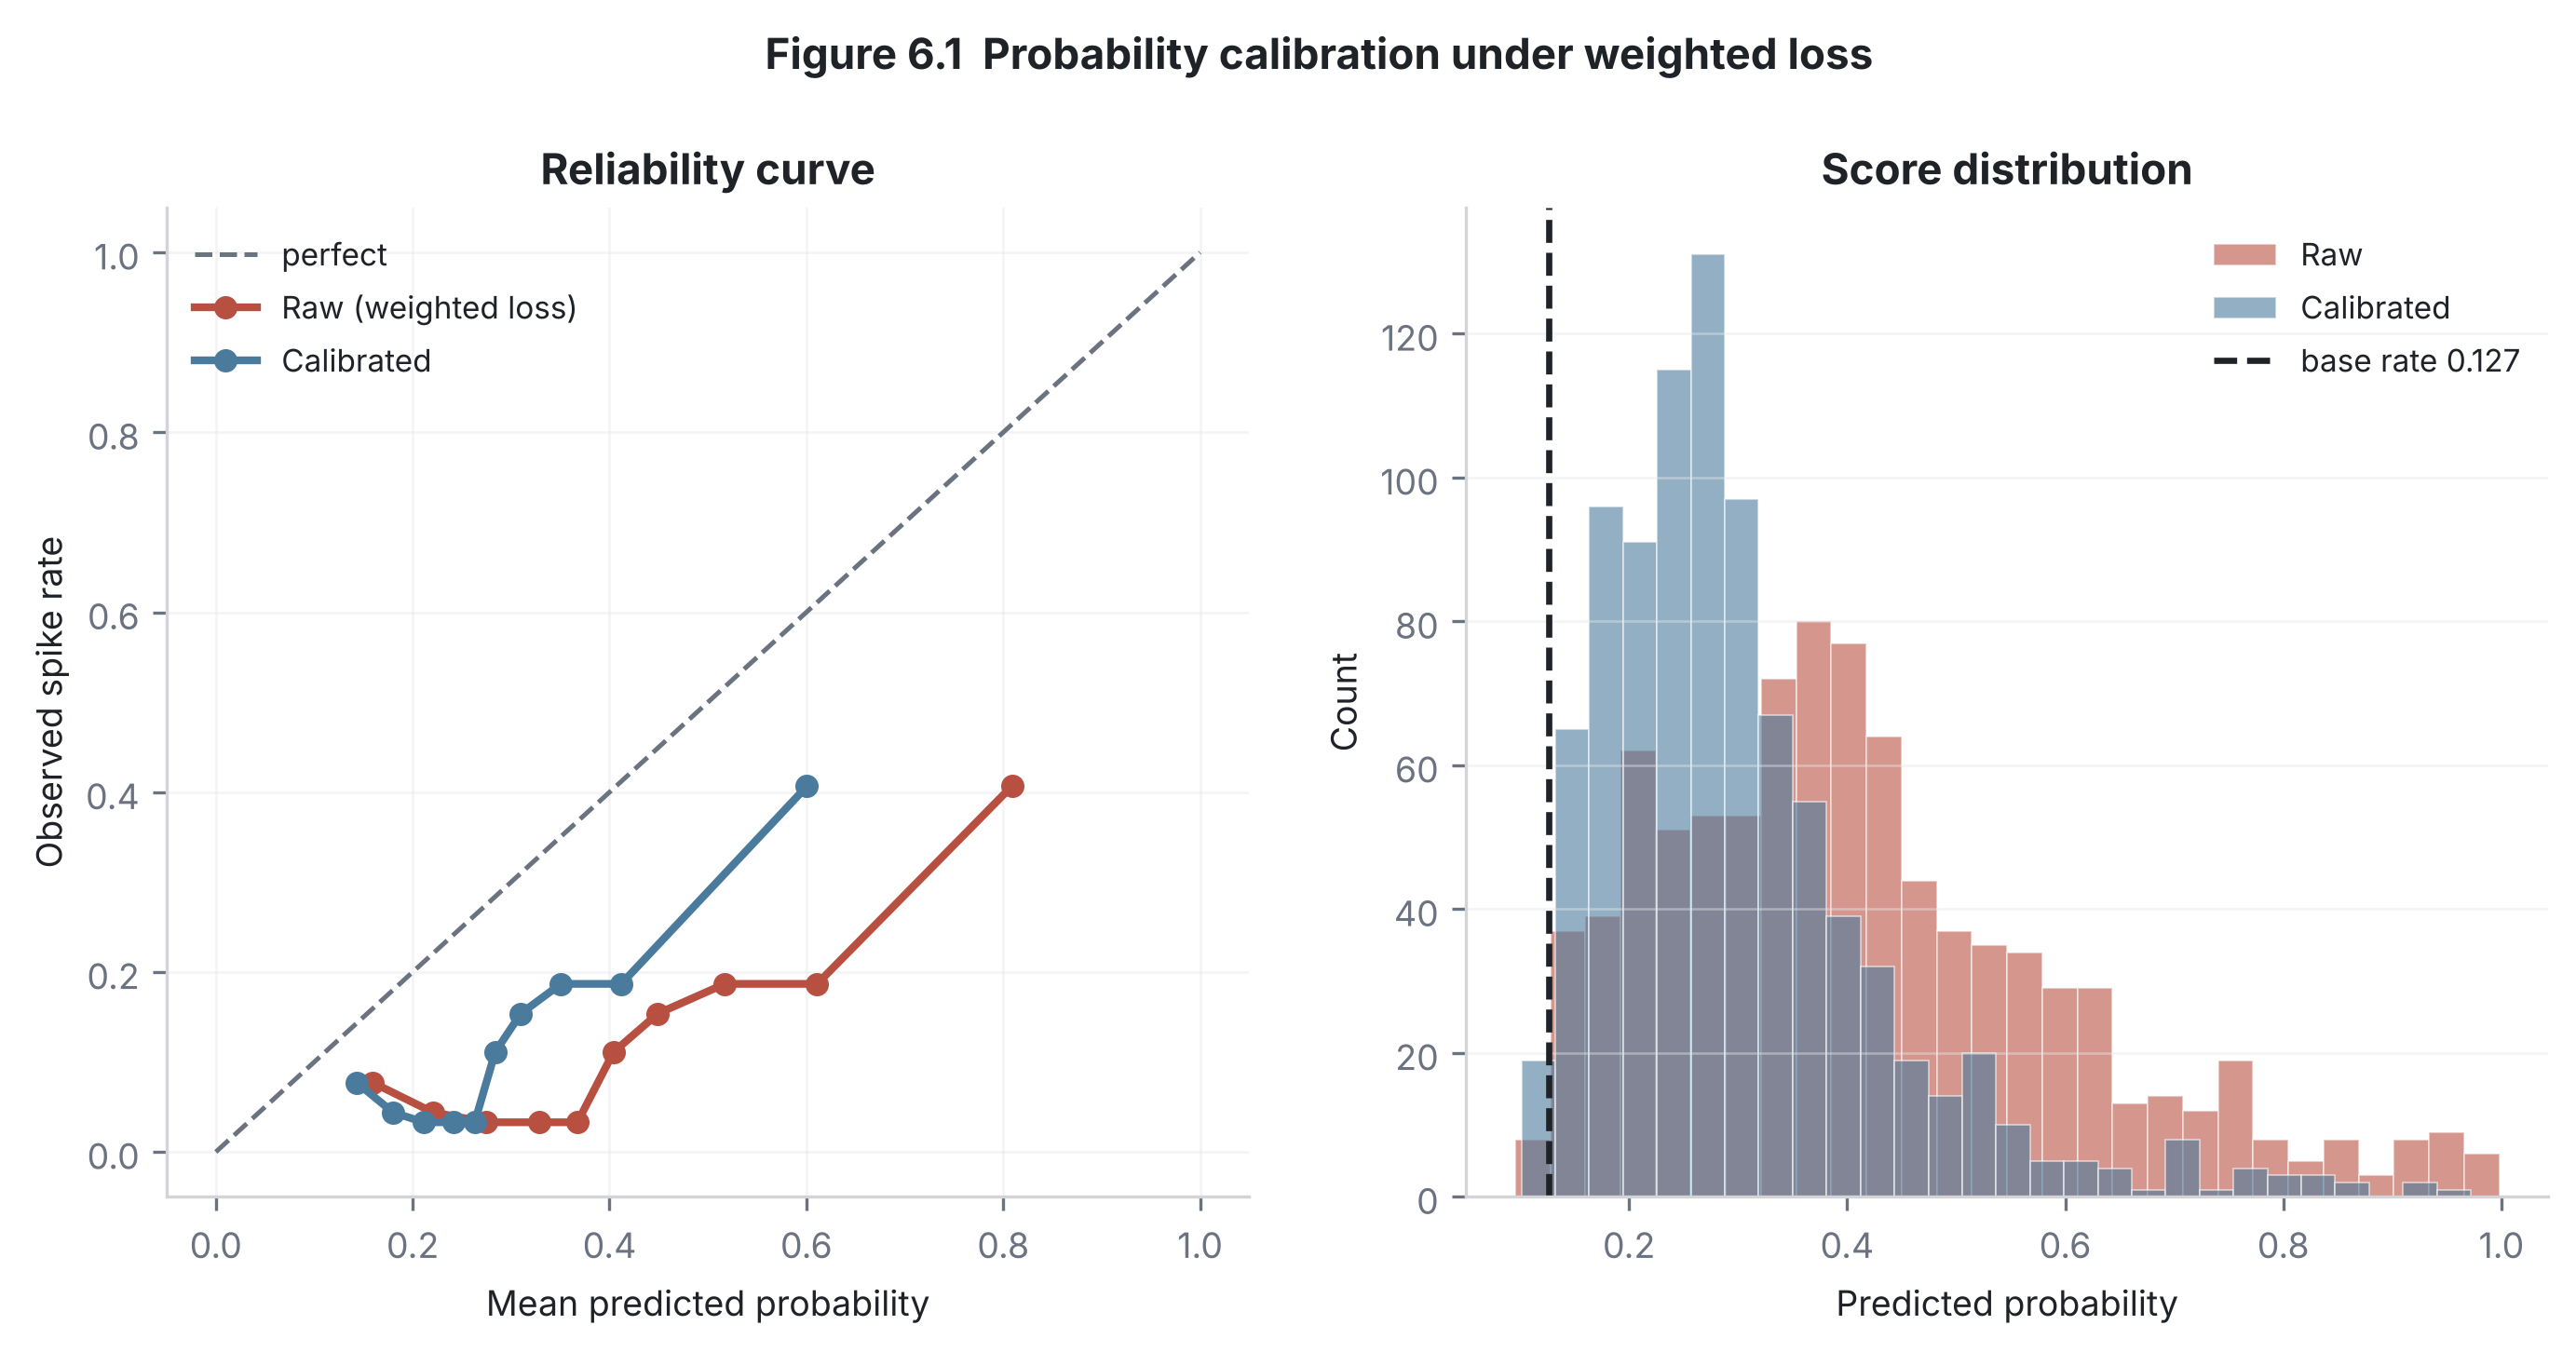
\includegraphics[width=\columnwidth]{fig6_1_calibration.png}}
\caption{Reliability curve and score distribution before and after Platt
scaling. The calibrated curve moves toward the diagonal without reaching it,
because the calibration partition carries a $34.88\%$ base rate against
$12.65\%$ in test.}
\label{fig:calib}
\end{figure}

\begin{table}[htbp]
\caption{Test partition results (base rate 0.127)}
\begin{center}
\begin{tabular}{@{}lrrrr@{}}
\toprule
\textbf{Model} & \textbf{Recall} & \textbf{Prec.} & \textbf{PR-AUC} & \textbf{P@50} \\
\midrule
Logistic regression & \textbf{0.852} & 0.186 & 0.356 & 0.460 \\
Gradient boosted trees & 0.513 & 0.196 & 0.301 & 0.500 \\
Seasonal persistence & 0.043 & 0.714 & --- & --- \\
\bottomrule
\end{tabular}
\label{tab:results}
\end{center}
\end{table}

Thresholds were selected on validation and the test partition scored once.
The recall target of 0.80 is met. The precision target of 0.60 is not, and
this is arithmetic rather than tuning failure: at a 12.7\% base rate, recovering
85\% of positives necessarily admits many false alarms. Precision@50 is the
operationally meaningful figure, since an agency acts on a ranked list under a
fixed budget; at 0.46 to 0.50 it represents roughly 3.8$\times$ lift over the
base rate. The seasonal baseline is precise but fires almost never, recovering
4.3\% of spikes, which is why recall is the primary metric.

\section{Model and Scope Selection}
\label{sec:models}

Preprocessing choices are only defensible against the estimator they feed, so
six candidates were compared on identical features and the same temporal
split, and two training scopes were tested against an identical test
partition. Both experiments are reproducible via
\texttt{python -m src.model\_selection}.

\begin{table}[htbp]
\caption{Candidate models, three northeastern states}
\begin{center}
\footnotesize
\begin{tabular}{@{}lrrrr@{}}
\toprule
\textbf{Model} & \textbf{Recall} & \textbf{PR-AUC} & \textbf{P@50} & \textbf{P@r$=$.80} \\
\midrule
Logistic (L2) & \textbf{0.835} & 0.356 & 0.46 & \textbf{0.228} \\
Logistic (ElasticNet) & 0.835 & 0.356 & 0.44 & 0.224 \\
Extra Trees & 0.635 & \textbf{0.386} & \textbf{0.62} & 0.173 \\
HistGradientBoosting & 0.600 & 0.374 & 0.54 & 0.170 \\
Random Forest & 0.600 & 0.358 & 0.60 & 0.163 \\
XGBoost & 0.504 & 0.301 & 0.50 & 0.140 \\
\bottomrule
\end{tabular}
\label{tab:models}
\end{center}
\end{table}

\textbf{Deviation 7.} Gradient boosting was the planned primary estimator, on
the conventional grounds that it is the standard choice for tabular
classification. It placed last of six on every metric
(Table~\ref{tab:models}). Logistic regression with an $L_2$ penalty exceeds it
by $0.33$ recall and by $0.088$ precision at the recall target. Extra Trees is
the strongest non-linear candidate, ahead of XGBoost by $28\%$ on PR-AUC.

The explanation is the structural break documented in
Section~\ref{sec:results}. Boosting fits residuals sequentially and has
sufficient capacity to model the pre-2023 price regime tightly, which does not
transfer across the subsidy removal and currency float. Extra Trees randomises
split thresholds as well as feature subsets, a stronger variance reduction
that degrades more gracefully under distribution shift. ElasticNet matched
$L_2$ to four decimal places, so the simpler penalty was retained.

\textbf{Selected: logistic regression ($L_2$) as primary, Extra Trees as the
non-linear comparison.}

\subsection{Why precision at matched recall decides this}

Figure~\ref{fig:models} shows why two reasonable summaries disagree. In the
left panel the tree models lead below recall $0.4$ and the linear models
overtake beyond roughly $0.6$. A model selected on PR-AUC or on precision@50
would therefore be selected on behaviour in a region the system never operates
in, because meeting a recall target of $0.80$ means working far down the
ranked list.

\begin{figure*}[htbp]
\centerline{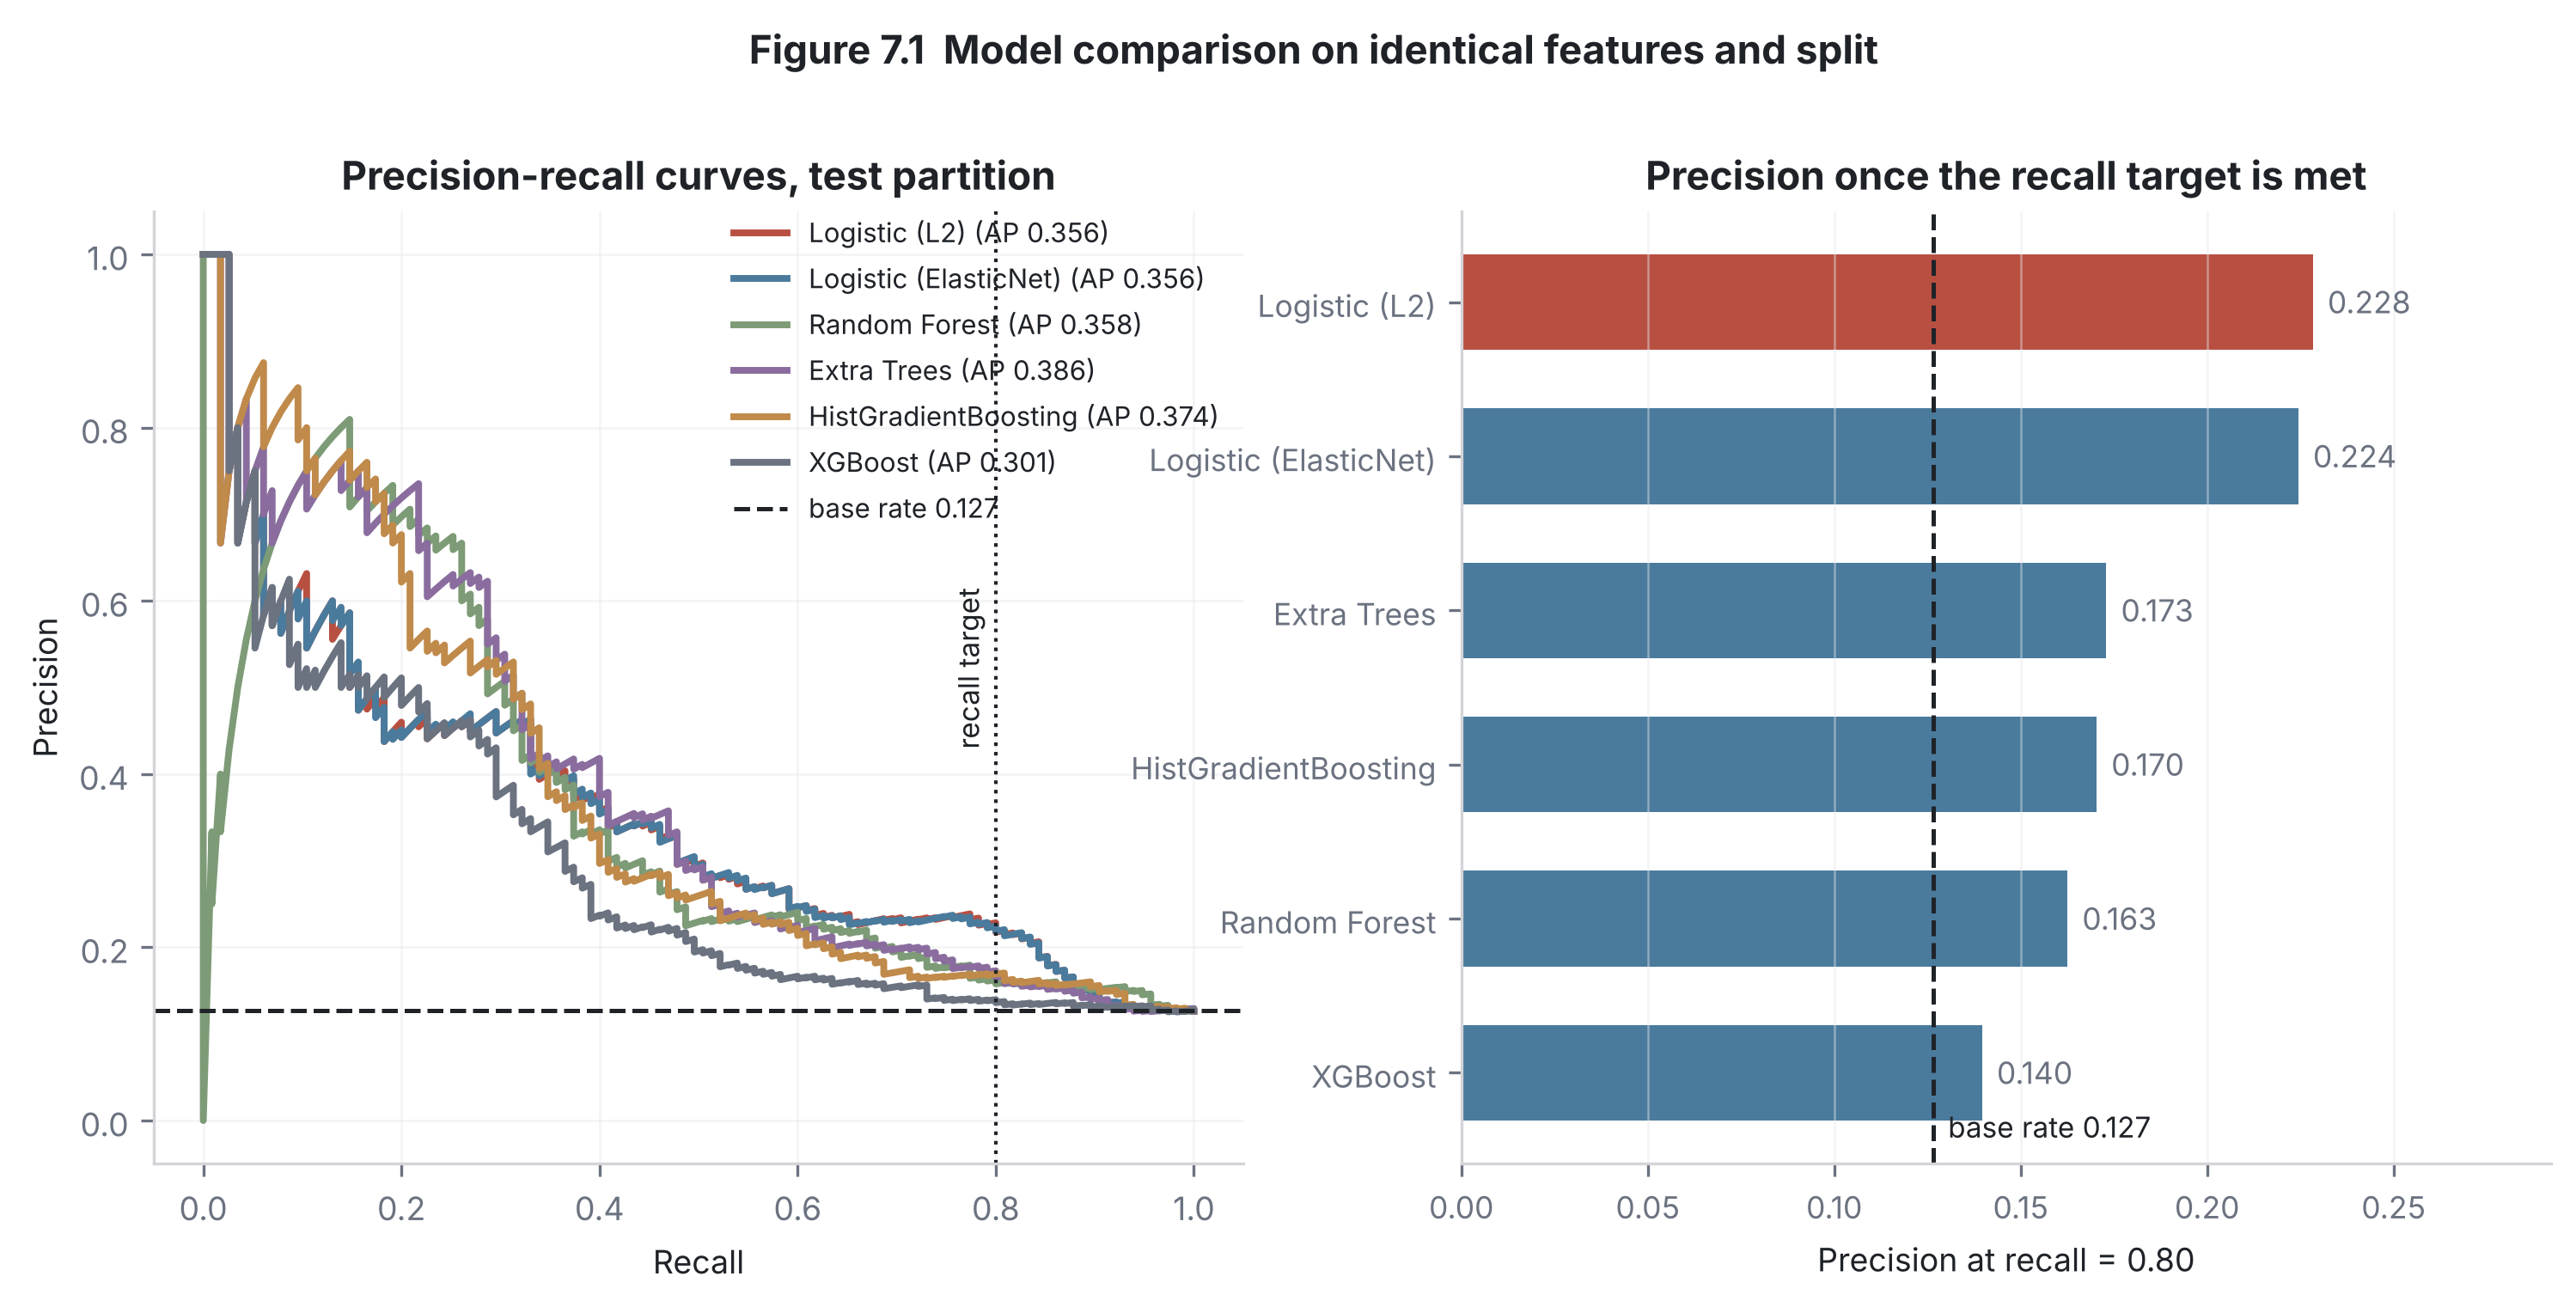
\includegraphics[width=0.88\textwidth]{fig7_1_model_comparison.png}}
\caption{Model comparison on identical features and split. Left: full
precision-recall curves, where tree models lead at low recall. Right:
precision read off at the stated recall target, which is where selection
happens. The two views disagree, and the right panel governs.}
\label{fig:models}
\end{figure*}

\subsection{Training scope}

Eleven further states exist in the source data but stop reporting in January
2023. Including them nearly doubles the training set, from 4{,}956 to
11{,}287 rows, and would additionally make geopolitical zone a non-constant
feature, since the three in-scope states all lie in the North East.

The headline metrics improve: PR-AUC rises from $0.356$ to $0.399$ and
precision@50 from $0.46$ to $0.62$, the latter meeting the stated precision
target. At matched recall the expansion is worse throughout the operating
region (Table~\ref{tab:scope}).

\begin{table}[htbp]
\caption{Precision at matched recall, by training scope}
\begin{center}
\begin{tabular}{@{}lrrr@{}}
\toprule
\textbf{Training scope} & \textbf{r$=$0.70} & \textbf{r$=$0.80} & \textbf{r$=$0.85} \\
\midrule
3 northeastern states & \textbf{0.239} & \textbf{0.228} & \textbf{0.190} \\
All 14 states & 0.190 & 0.179 & 0.145 \\
\bottomrule
\end{tabular}
\label{tab:scope}
\end{center}
\end{table}

The expanded model ranks its top fifty better and degrades faster below that.
Since the system is specified by a recall target rather than a fixed alert
budget, the narrower scope is retained. Grouping states by geopolitical zone
was considered and rejected for the same scoping reason: within the selected
three states the zone label is constant and carries no information.

\textbf{On augmentation.} No synthetic augmentation is applied. The label is
derived from the price series, so SMOTE or time-series warping would perturb
prices and thereby perturb the labels they are intended to preserve. Real
data expansion was tested instead, with the result above.

\clearpage
\section{Strategy versus Reality Decision Log}
\label{sec:log}

Table~\ref{tab:decisionlog} sets each planned preprocessing choice against
what implementation required, with the statistic or figure that settled it.
Nine steps executed as planned. Four did not, and in every case the change was
forced by a measurement rather than by convenience: a mechanism diagnosis that
produced unusable features, a predicted collinearity problem that did not
materialise, a dimensionality assumption contradicted by the variance profile,
and an estimator chosen by convention that lost to a simpler alternative on
every metric.

\begin{table*}[!t]
\caption{Planned strategy against executed implementation}
\begin{center}
\small
\begin{tabular}{@{}p{2.6cm}p{3.8cm}p{3.8cm}p{6.2cm}@{}}
\toprule
\textbf{Step} & \textbf{Planned} & \textbf{Executed} & \textbf{Evidence} \\
\midrule
Missingness
& 4 MNAR indicators
& 2 retained, 2 dropped
& Constant in modelled rows; Little's $p<0.001$ (Fig. 1.1) \\
\addlinespace
Imputation
& Median; 1-month interpolation
& As planned
& Skew $23.47$; 356 rows filled \\
\addlinespace
Outliers
& IQR flag, no price capping
& As planned
& Flagged precede spike 21.4\% vs 16.3\% (Fig. 2.1) \\
\addlinespace
Ratio capping
& 1st/99th pct
& As planned
& \texttt{mom\_1m} skew $32.72$ \\
\addlinespace
Collinearity
& Severe expected; $|\rho|\!\geq\!0.85$ + VIF
& 1 pair only; VIF decisive
& $\rho=0.876$; VIF $10.52\!\to\!6.72$ (Fig. 3.1--3.3) \\
\addlinespace
Encoding
& Target encoding for commodity
& Built, not deployed
& Cardinality 37 after scoping \\
\addlinespace
Scaling
& Standard (linear) / none (trees)
& As planned
& Skew $23.47\!\to\!-0.21$ (Fig. 4.1) \\
\addlinespace
PCA
& Expected PC1 dominance
& 10 PCs for 90\%
& PC1 $=29.6\%$ (Fig. 5.1) \\
\addlinespace
Split
& Chronological 70/15/15
& As planned
& Group-respecting by construction \\
\addlinespace
Fold features
& Rebuild per fold
& Unnecessary
& Backward windows under date cut \\
\addlinespace
Imbalance
& Weighted loss
& Weighted loss + Platt
& Brier $0.187\!\to\!0.126$ (Fig. 6.1) \\
\addlinespace
Estimator
& Gradient boosting primary
& Logistic $L_2$ + Extra Trees
& XGBoost last of six; $0.140$ vs $0.228$ P@r$=$.80 (Fig. 7.1) \\
\addlinespace
Scope
& 3 states
& 3 states retained
& 14-state expansion worse at matched recall \\
\bottomrule
\end{tabular}
\label{tab:decisionlog}
\end{center}
\end{table*}

\section{Conclusion}

Seven deviations arose during execution, and the pattern among them is
instructive. Two corrected over-confident predictions about the data
(collinearity severity, PCA dominance). One corrected an over-cautious
methodological commitment (per-fold feature rebuilding). One discovered that a
correct diagnosis had produced unusable features (constant missingness
indicators). One was a genuine omission (probability calibration). One was an
unplanned empirical finding that strengthened the design rationale (the
regime break visible in partition class balance). The last overturned a
default inherited from convention rather than from evidence: gradient boosting
was the planned estimator and proved the weakest of six tested.

None required abandoning a planned decision because it was inconvenient, and
the three decisions most likely to be questioned, retaining extreme price
values, declining to stratify the split, and rejecting gradient boosting, are
the three with the strongest numerical support.

Three items carry forward: SHAP attribution for per-prediction explanation;
refitting the calibrator with each rolling window, since the calibration
partition carries a 34.88\% base rate against 12.65\% in test and a mapping
learned at one base rate transfers imperfectly; and acquisition of exchange
rate and state-level fuel series to represent the structural break as an
observable input rather than an unexplained regime.

\section*{Reproducibility}

All statistics in this report are regenerated by
\texttt{python -m src.run\_diagnostics}, which writes
\texttt{data/processed/diagnostics.json}. The execution notebook runs end to
end from the raw file. Source, figures and reports are available at
\url{https://github.com/nimatsadiq/AISD_proj_F26}.

\begin{thebibliography}{00}

\bibitem{little1988} R.~J.~A. Little, ``A test of missing completely at random
for multivariate data with missing values,'' \emph{Journal of the American
Statistical Association}, vol.~83, no.~404, pp.~1198--1202, 1988.

\bibitem{bergsma2013} W. Bergsma, ``A bias-correction for Cram\'{e}r's $V$ and
Tschuprow's $T$,'' \emph{Journal of the Korean Statistical Society}, vol.~42,
no.~3, pp.~323--328, 2013.

\bibitem{tukey1977} J.~W. Tukey, \emph{Exploratory Data Analysis}. Reading,
MA, USA: Addison-Wesley, 1977.

\bibitem{platt1999} J. Platt, ``Probabilistic outputs for support vector
machines and comparisons to regularized likelihood methods,'' in
\emph{Advances in Large Margin Classifiers}, Cambridge, MA, USA: MIT Press,
1999, pp.~61--74.

\bibitem{chawla2002} N.~V. Chawla, K.~W. Bowyer, L.~O. Hall, and W.~P.
Kegelmeyer, ``SMOTE: Synthetic minority over-sampling technique,''
\emph{Journal of Artificial Intelligence Research}, vol.~16, pp.~321--357,
2002.

\bibitem{chen2016} T. Chen and C. Guestrin, ``XGBoost: A scalable tree
boosting system,'' in \emph{Proc. 22nd ACM SIGKDD Int. Conf. Knowledge
Discovery and Data Mining}, San Francisco, CA, USA, 2016, pp.~785--794.

\bibitem{hyndman2021} R.~J. Hyndman and G. Athanasopoulos,
\emph{Forecasting: Principles and Practice}, 3rd ed. Melbourne, Australia:
OTexts, 2021.

\bibitem{wfp2026} World Food Programme, ``Nigeria food prices,'' WFP
Vulnerability Analysis and Mapping Price Database, Humanitarian Data Exchange,
2026. [Online]. Available:
\url{https://data.humdata.org/dataset/wfp-food-prices-for-nigeria}

\end{thebibliography}

\end{document}
